\section{The Colony-Wise PV Module Model}
\subsection{The Colony-Wise Model Equivalent Circuit Diagram}
\begin{figure}[tb]
    \centering
    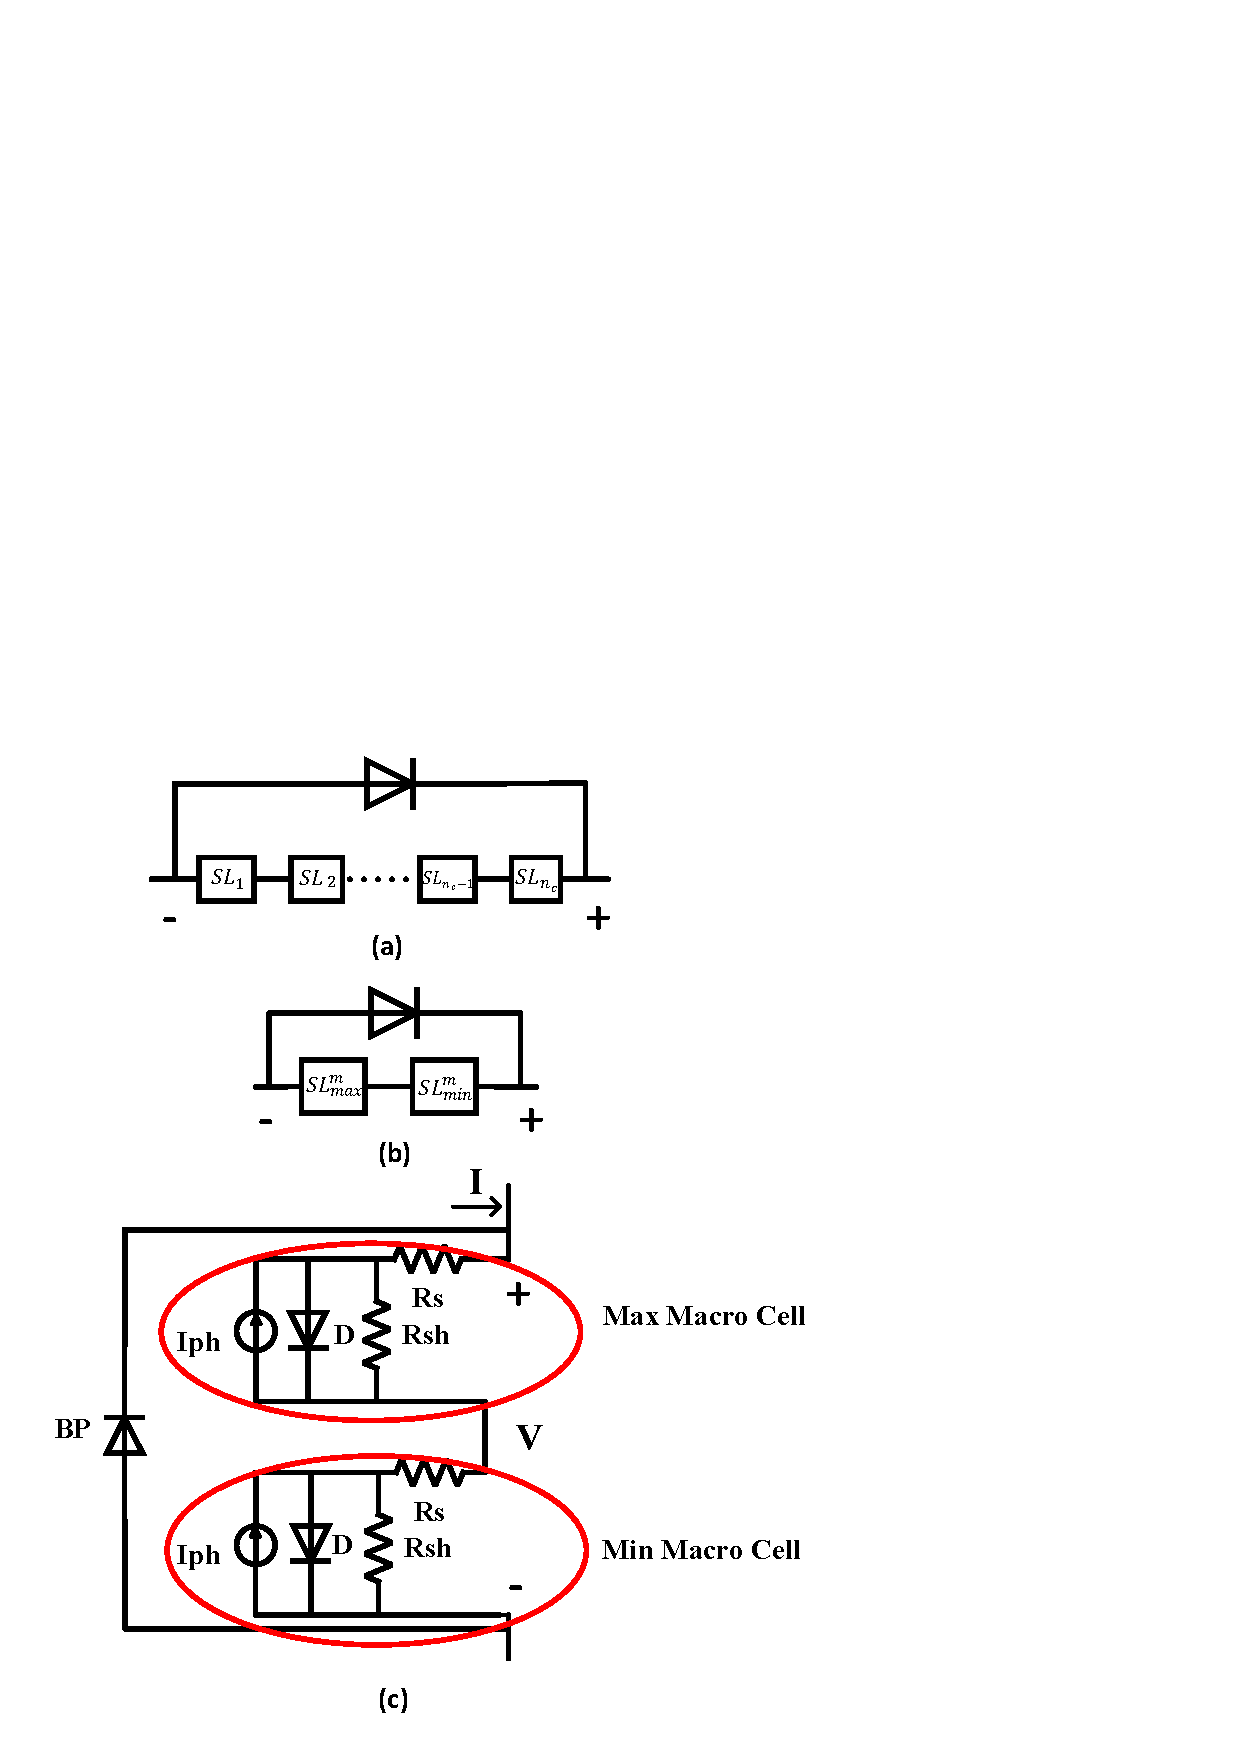
\includegraphics[width=1\columnwidth]{figs/cw_model_diagram.pdf}
    \caption{(a) One colony with $n_c$ solar cells (b) One colony model in Colony-Wise model (c) Circuit diagram of a colony modeled by the Colony-Wise Model}
    \label{fig:cwDiagram}
\end{figure}

One colony in a PV module can be represented as in Figure \ref{fig:cwDiagram} (a) abstractly. Let us assume that this colony has $n_c$ solar cells. $SL_1$ to $SL_{n_c}$ denotes shading level of each solar cell. Recall that the Ground Truth model models each solar cell with a One-Diode model. Differ from the GT model, in the Colony-Wise model, all $n_c$ solar cells are lumped into at most two macro cells as shown in Figure \ref{fig:cwDiagram} (b). If $SL_1 = SL_2 = \dots = SL_{n_c}$, there is only one macro cell. Then all of the $n_c$ solar cells are lumped into this macro cell. Otherwise, all cells are lumped into two macro cells according to their shading levels (SLs). The two macro cells are also modeled by the One-Diode model, with their shading levels as $SL_{max}^m$ and $SL_{min}^m$. The superscript $m$ denotes the parameters are from macro cells. Section III B details the generation of parameters of the Colony-Wise model from the Ground Truth model. $SL_{max}^m$ and $SL_{min}^m$ are defined as the following:
\begin{equation}\label{equ:slMax}
  SL_{max}^m = \max_{i \in n_c}{\{SL_1, SL_2,  \dots, SL_{n_c} \}}
\end{equation}
\begin{equation}\label{equ:slMin}
  SL_{min}^m = \min_{i \in n_c}{\{SL_1, SL_2,  \dots, SL_{n_c} \}}
\end{equation}

\subsection{Parameter Generation of The Colony-Wise Model}
Heuristically, we pick the two most representative solar cells within each colony to build the Colony-Wise model. These two cells are the basis of the two macro cells - the Max Macro Cell and the Min Macro Cell. The two macro cells are circled in the Figure \ref{fig:cwDiagram} (c). One cell ( to build the Max Macro Cell) has the maximum shading level $SL_{max}^m$, while the other cell (to build the Min Macro Cell) has the minimum shading level $SL_{min}^m$.

$n_{max}$ and $n_{min}$  counts the numbers of cells that belong to each macro cells within one colony. Note that:
\begin{equation}\label{equ:minMaxEqu}
  n_{max} + n_{min} = n_c
\end{equation}

The belonging of a cell depends on the comparison between its shading level and the threshold. The threshold is defined in Equation \ref{equ:thres}:
\begin{equation}\label{equ:thres}
  thres = \frac{1}{2}(SL_{max}^m+ SL_{min}^m )
\end{equation}
For a solar cell, if its $SL \ge thres$, it belongs to the Max Macro Cell; otherwise, it belongs to the Min Macro Cell.

The circuit diagram of a colony modeled by the Colony-Wise model is as shown in Figure \ref{fig:cwDiagram} (c). We can derive the parameters of the Max Macro Cell and the Min Macro Cell based on $n_{max}$ and $n_{min}$. The model reduction is shown in Table \ref{table:cwRule}.

\begin{table}[tb]
  \caption{Model Reduction Rule for the Colony-Wise Model }
  \label{table:cwRule}
  \centering
  \normalsize
\begin{tabular}{|l|l|l|}
  \hline
  Parameter & Max Macro Cell & Min Macro Cell \\
  \hline
  $I_{ph}^m$ & $SL_{max}^m$ & $SL_{min}^m$ \\
  \hline
  $I_s^m$ & $I_{s_o}$ & $I_{s_o}$ \\
  \hline
  $N^m$ & $n_{max}*N_o$ & $n_{min}*N_o$ \\
  \hline
  $R_s^m$ & $n_{max}*R_{s_o}$ & $n_{min}*R_{s_o}$ \\
  \hline
  $R_{sh}^m$ & $R_{sh_o}$ & $R_{sh_o}$ \\
  \hline
\end{tabular}
\end{table}

\subsection{Computational Complexity of the Colony-Wise Model}
The circuit solver spends most of its time on solving non-linear equations. Therefore, the non-linear components, which are the diodes in PV module models, dominate the computational time. For an $mSnP$ PV module with $n_{bp}$ bypass diodes for each chain, the ratio of number of diodes between the GT model and CW model is:
\begin{equation}\label{equ:diodeRatioGTCW}
  diode\_ratio = \frac{m*n+n*n_{bp}}{n*n_{bp}*3}
\end{equation}





